\documentclass[12pt]{article}

% ===== Configuración común =====
\newcommand{\commonpath}{../../common}
% ===== Idioma y codificación =====
\usepackage[spanish, es-nodecimaldot]{babel}
\usepackage[utf8]{inputenc}
\usepackage[T1]{fontenc}
\usepackage{textcomp}

% ===== Tipografía moderna =====
\usepackage{helvet}
\renewcommand{\familydefault}{\sfdefault}
\usepackage{microtype}
\usepackage{xcolor}

% ===== Márgenes y formato =====
\usepackage[a4paper,top=2.8cm,bottom=2.8cm,left=3cm,right=3cm]{geometry}
\usepackage{titlesec}
\titleformat{\section}{\Large\bfseries}{\thesection.\ }{0.4em}{}
\titleformat{\subsection}{\large\bfseries}{\thesubsection.\ }{0.4em}{}
\titlespacing*{\section}{0pt}{1.6ex plus .5ex minus .2ex}{1.0ex}
\titlespacing*{\subsection}{0pt}{1.2ex plus .5ex minus .2ex}{0.7ex}

% ===== Colores =====
\definecolor{UMABlue}{RGB}{0,51,102}

% ===== Paquetes útiles =====
\usepackage{amsmath}
\usepackage{amssymb}
\usepackage{graphicx}
\usepackage{booktabs}
\usepackage{tabularx}
\usepackage{siunitx}
\usepackage{float}
\usepackage{enumitem}
\usepackage{listings}
\usepackage[hidelinks]{hyperref}
\usepackage{tikz}
\usetikzlibrary{arrows.meta, decorations.markings, patterns}
\sisetup{locale=DE}

% ===== Estilo para listados de código =====
\lstset{
  language=C++,
  basicstyle=\ttfamily\footnotesize,
  keywordstyle=\bfseries\color{UMABlue},
  commentstyle=\itshape\color{gray},
  stringstyle=\color{red!60!black},
  numbers=left,
  numberstyle=\tiny\color{gray},
  numbersep=6pt,
  frame=single,
  framerule=0.4pt,
  rulecolor=\color{gray!50},
  breaklines=true,
  tabsize=4,
  showstringspaces=false,
  captionpos=b,
  aboveskip=8pt,
  belowskip=6pt,
}

% ===== Comandos personalizados — Ampliación de Robótica =====

% --- Abreviaturas frecuentes ---
\newcommand{\ros}{ROS~2}
\newcommand{\roshumble}{ROS~2 Humble}
\newcommand{\coppelia}{CoppeliaSim}
\newcommand{\pioneer}{Pioneer P3DX}

% --- Unidades ---
\newcommand{\ms}{\si{\meter\per\second}}
\newcommand{\hz}[1]{\SI{#1}{\hertz}}
\newcommand{\rad}{\si{\radian}}

% --- Pendiente (texto rojo para secciones por completar) ---
\newcommand{\pendiente}[1]{\textcolor{red}{\textbf{[PENDIENTE:} #1\textbf{]}}}

% ===== Portada reutilizable =====
% Uso: \portada{LAB-ID}{Título}{Subtítulo}
\newcommand{\portada}[3]{%
  {%
    \pagecolor{UMABlue}%
    \color{white}%
    \thispagestyle{empty}%
    \begin{center}
      \vspace*{0.8cm}
      
\includegraphics[width=0.22\textwidth]{\commonpath/img/logo_uma.png}\\[0.5cm]
      {\large UNIVERSIDAD DE MÁLAGA\\[0.3cm]}
      {\small Grado en Ingeniería Electrónica, Robótica y Mecatrónica\\[1.2cm]}
      {\huge\bfseries Memoria de Práctica\\[0.6cm]}
      {\LARGE\bfseries #1\\[0.2cm]}
      {\Large\bfseries #2\\[0.4cm]}
      {\normalsize\itshape #3\\[1.8cm]}
      {\normalsize Ampliación de Robótica\\[0.8cm]}
      {\large
        Saúl Gutiérrez Rodríguez\\[0.15cm]
        Pablo Haro García\\[0.15cm]
        Mario Merino Prado\\[0.8cm]
      }
      \rule{0.55\textwidth}{0.4pt}\\[0.3cm]
      {\small
        Repositorio: \texttt{github.com/marioomerino24/ampliacion\_robotica}\\[0.1cm]
        Entorno: \roshumble{} · \coppelia{} · \pioneer{}
      }
    \end{center}
    \clearpage
  }%
  \nopagecolor%
  \color{black}%
}

\graphicspath{{figures/}{\commonpath/img/}}

% ===== Documento =====
\begin{document}

\portada{Lab-MR 1-I}{Seguimiento de caminos expl\'{i}citos}%
        {Navegaci\'{o}n punto a punto con control proporcional}

\tableofcontents
\clearpage


% =====================================================================
%  1. OBJETIVO
% =====================================================================
\section{Objetivo}
Completar el m\'{e}todo \texttt{controlLoop()} del nodo \texttt{nav\_p2p.cpp} (paquete \texttt{seg\_tray}) para que el robot \pioneer{} simulado en \coppelia{} recorra una secuencia de waypoints definida en \texttt{nav\_params.yaml} mediante navegaci\'{o}n punto a punto con control proporcional de rumbo. Una vez verificado el recorrido completo, modificar la ganancia $K$ y comentar c\'{o}mo influye en la trayectoria del robot.


% =====================================================================
%  2. IMPLEMENTACIÓN
% =====================================================================
\section{Implementaci\'{o}n}

El nodo \texttt{nav\_p2p\_node} ya proporcionado en \texttt{seg\_tray} se encarga de cargar los waypoints del YAML, suscribirse a \texttt{/PioneerP3DX/odom} y publicar en \texttt{/PioneerP3DX/cmd\_vel} a 40~Hz. Lo \'{u}nico que hay que completar es el bloque indicado dentro de \texttt{controlLoop()} con las ecuaciones del enunciado. Las decisiones no obvias son:

\paragraph{Cambio a coordenadas locales del veh\'{i}culo.} El error de orientaci\'{o}n $\phi_e$ se obtiene m\'{a}s directamente expresando el waypoint en el sistema de referencia del robot. Aplicando la rotaci\'{o}n del enunciado:
\begin{equation*}
  x_{P_l} = \cos\phi_o\,(x_P - x) + \sin\phi_o\,(y_P - y), \qquad
  y_{P_l} = -\sin\phi_o\,(x_P - x) + \cos\phi_o\,(y_P - y),
\end{equation*}
queda $\phi_e = \operatorname{atan2}(y_{P_l},\, x_{P_l})$, que ya est\'{a} en el rango correcto sin necesidad de normalizaciones expl\'{i}citas.

\paragraph{Control proporcional y cinem\'{a}tica inversa.} La curvatura comandada es $\gamma = K\,\phi_e$ y las velocidades angulares de cada rueda se obtienen aplicando directamente las ecuaciones del enunciado:
\begin{equation*}
  \omega_i = \frac{v\,(1 - K\,\gamma)}{R}, \qquad
  \omega_d = \frac{v\,(1 + K\,\gamma)}{R}.
\end{equation*}
A partir de $(\omega_i, \omega_d)$ se recuperan las velocidades del veh\'{i}culo $(v, \omega)$ con la cinem\'{a}tica directa y se publican en \texttt{cmd\_vel}.

\paragraph{Cambio de waypoint a $\SI{1}{\meter}$.} El waypoint se considera alcanzado cuando $\sqrt{(x_P - x)^2 + (y_P - y)^2} < \SI{1}{\meter}$, tal y como indica el enunciado, y se pasa al siguiente. Cuando no quedan waypoints, se publica $v = \omega = 0$.


% =====================================================================
%  3. PRUEBAS
% =====================================================================
\section{Pruebas}

Tras lanzar la escena \texttt{p2p\_scene.ttt} en \coppelia{} y ejecutar \texttt{ros2 launch seg\_tray nav\_p2p\_launch.py}, el robot recorre los $7$ waypoints del fichero de configuraci\'{o}n a $v = \SI{1.2}{\meter\per\second}$ y completa el camino. La Figura~\ref{fig:p2p_recorrido} muestra el recorrido sobre el plano del simulador.

\begin{figure}[H]
  \centering
  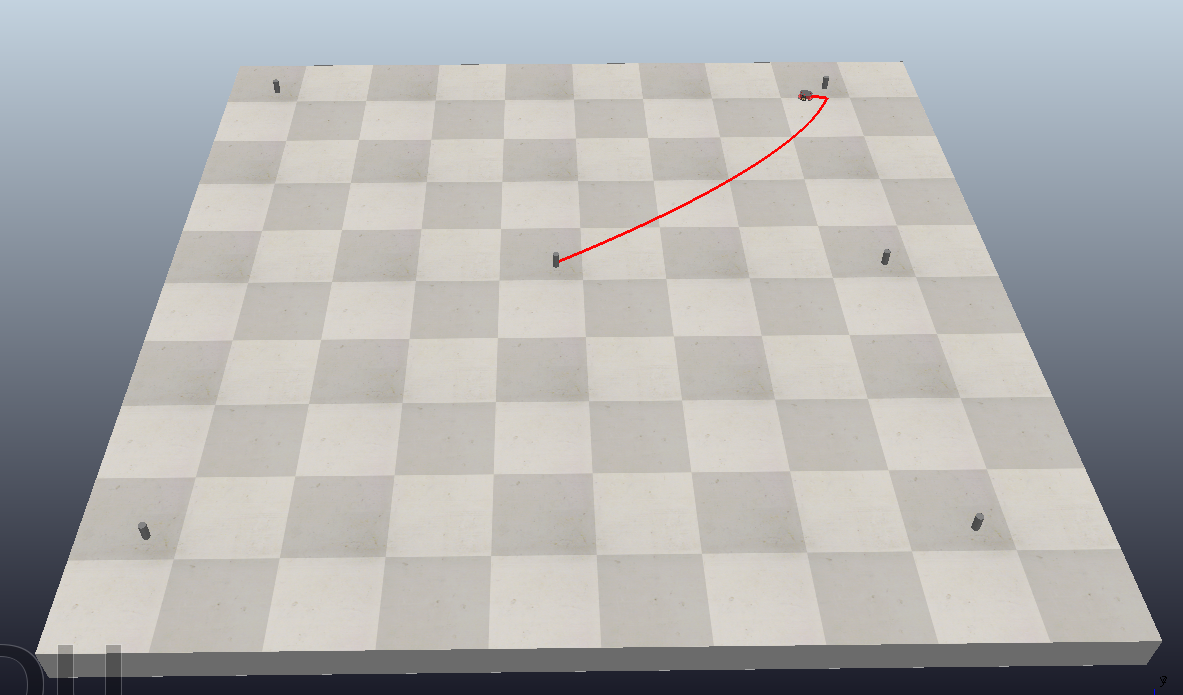
\includegraphics[width=0.9\linewidth]{figure1_p1_1}
  \caption{Recorrido rectangular del \pioneer{} con control P2P en \coppelia{}.}
  \label{fig:p2p_recorrido}
\end{figure}

\subsection{Influencia de la ganancia $K$}
El enunciado pide modificar la ganancia y comentar el efecto sobre la trayectoria:
\begin{itemize}[leftmargin=2em]
  \item Con $K$ \textbf{peque\~{n}o} (e.g.\ $K = 1$) el robot corrige el rumbo lentamente y se aleja lateralmente del waypoint antes de orientarse, dibujando arcos amplios entre puntos consecutivos.
  \item Con $K$ \textbf{moderado} (e.g.\ $K = 4$) la respuesta es r\'{a}pida y la trayectoria entre waypoints es pr\'{a}cticamente recta, con curvas suaves en los cambios de waypoint.
  \item Con $K$ \textbf{grande} (e.g.\ $K \gtrsim 6$) la curvatura comandada se vuelve excesiva y aparecen oscilaciones porque el error angular cambia de signo de un ciclo al siguiente.
\end{itemize}

El valor $K = 4$ ofrece un buen compromiso entre rapidez y estabilidad para este recorrido.


% =====================================================================
%  4. COMENTARIOS FINALES
% =====================================================================
\section{Comentarios finales}

El controlador implementado cumple lo que pide el enunciado: el robot sigue la secuencia de waypoints con control proporcional sobre el error de orientaci\'{o}n calculado en coordenadas locales, y la ganancia $K$ act\'{u}a como esperado seg\'{u}n el an\'{a}lisis del par\'{a}metro. La estructura del nodo proporcionado ($\SI{1.2}{\meter\per\second}$, periodo $\SI{25}{\milli\second}$, tolerancia $\SI{1}{\meter}$) es suficiente para completar el recorrido en el escenario sin obst\'{a}culos.

\end{document}
